\begin{comment}
try a scan and fill for fill array?
\end{comment}

%==========================================================================

\begin{frame}[fragile]

  {\Huge Hierarchical parallelism}

  \vspace{10pt}

  {\large Finding and exploiting more parallelism in your computations.}

  \vspace{20pt}

  \textbf{Learning objectives:}
  \begin{itemize}
    \item {Similarities and differences between outer and inner levels of parallelism}
    \item {Thread teams (league of teams of threads)}
    \item {Performance improvement with well-coordinated teams}
  \end{itemize}

  \vspace{-20pt}

\end{frame}

%==========================================================================

\begin{frame}[fragile]{Example: inner product (0)}

  \ul{\textbf{(Flat parallel) Kernel:}}

  \vspace{-3pt}

  \begin{code}[keywords={}]
Kokkos::parallel_reduce("yAx",N,
  KOKKOS_LAMBDA (const int row, double & valueToUpdate) {
    double thisRowsSum = 0;
    for (int col = 0; col < M; ++col) {
      thisRowsSum += @blueA@blue(row,col) * @darkgreenx@darkgreen(col);
    }
    valueToUpdate += @darkredy@darkred(row) * thisRowsSum;
  }, @orangeresult@orange);
  \end{code}

 \begin{tikzpicture}[remember picture, overlay]
    \node [shift={(-8.0cm,1.10cm)}]  at (current page.south east)
      {%
      \begin{tikzpicture}[remember picture, overlay]
        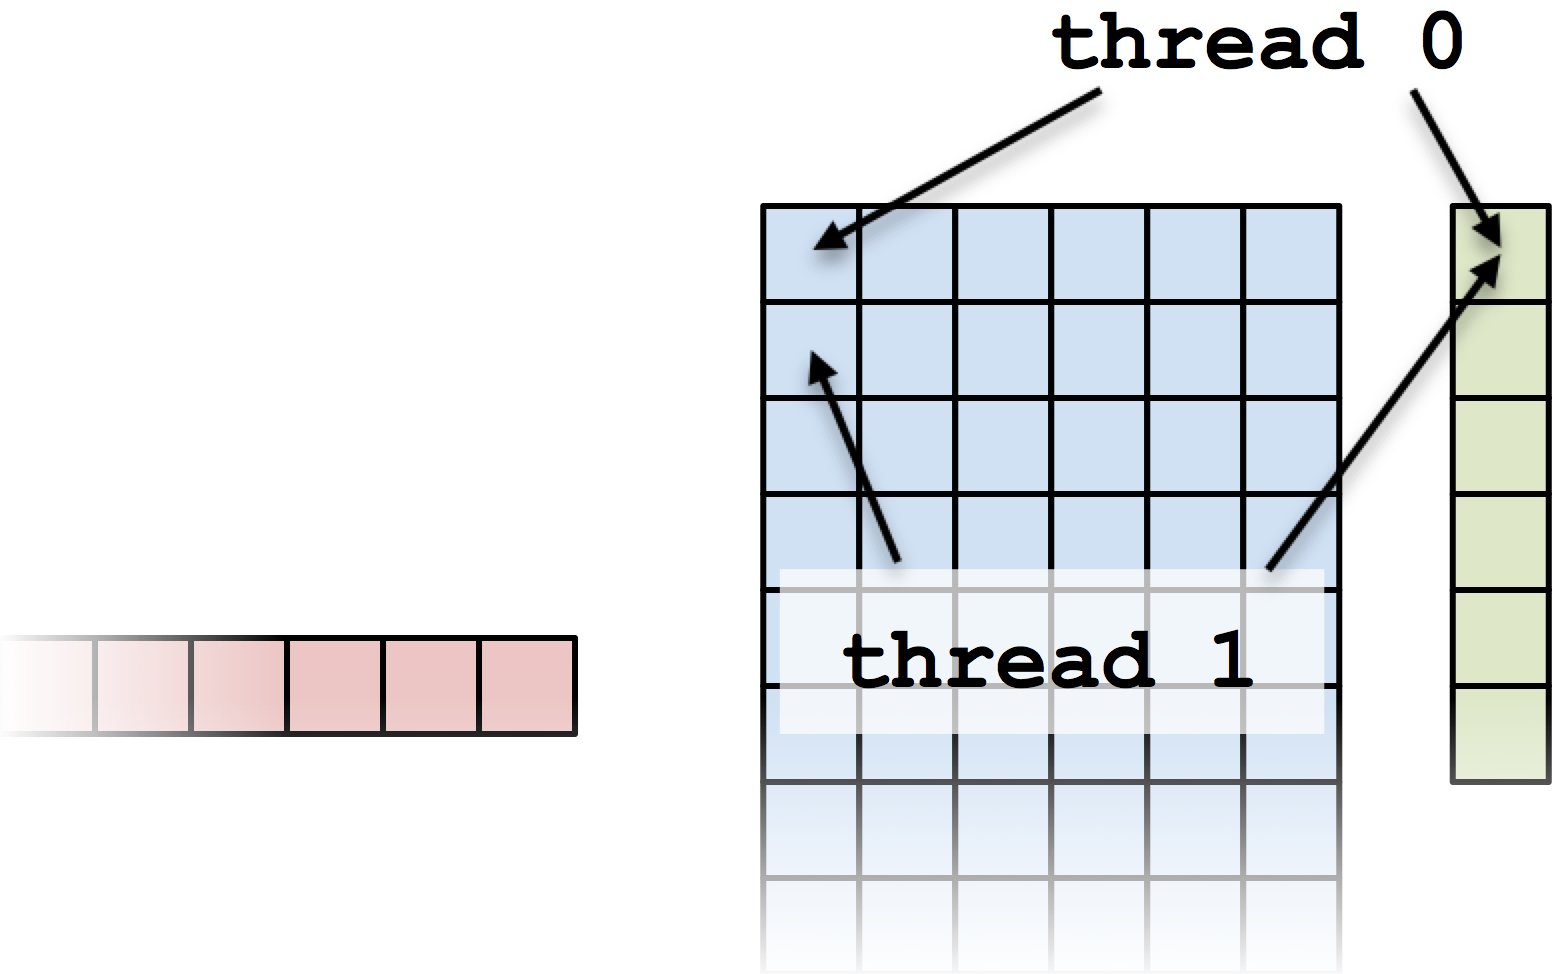
\includegraphics[width=0.60\textwidth]{figures/InnerProductExample_Flat}
      \end{tikzpicture}
      };
  \end{tikzpicture}

  \vspace{10pt}
  \pause

  \begin{columns}[t,onlytextwidth]
    \column{.60\textwidth}
    \textbf{Problem:} What if we don't have enough rows to saturate the GPU?
    \column{.40\textwidth}
  \end{columns}

  \vspace{10pt}
  \pause

  \textbf{Solutions?}
  \pause
  \vspace{-5pt}

  \begin{itemize}
    \item{Atomics}
    \item{Thread teams}
  \end{itemize}

\end{frame}

%==========================================================================
\iffull
\begin{frame}[fragile]{Example: inner product (1)}

  \ul{\textbf{Atomics kernel:}}

  \vspace{-3pt}

  \begin{code}[keywords={}]
Kokkos::parallel_for("yAx", N*M,
  KOKKOS_LAMBDA (const size_t index) {
    const int row = extractRow(index);
    const int col = extractCol(index);
    atomic_add(&@orangeresult@orange, @redy@red(row) * @blueA@blue(row,col) * @darkgreenx@darkgreen(col));
  });
  \end{code}

 \begin{tikzpicture}[remember picture, overlay]
    \node [shift={(-8.0cm,1.10cm)}]  at (current page.south east)
      {%
      \begin{tikzpicture}[remember picture, overlay]
        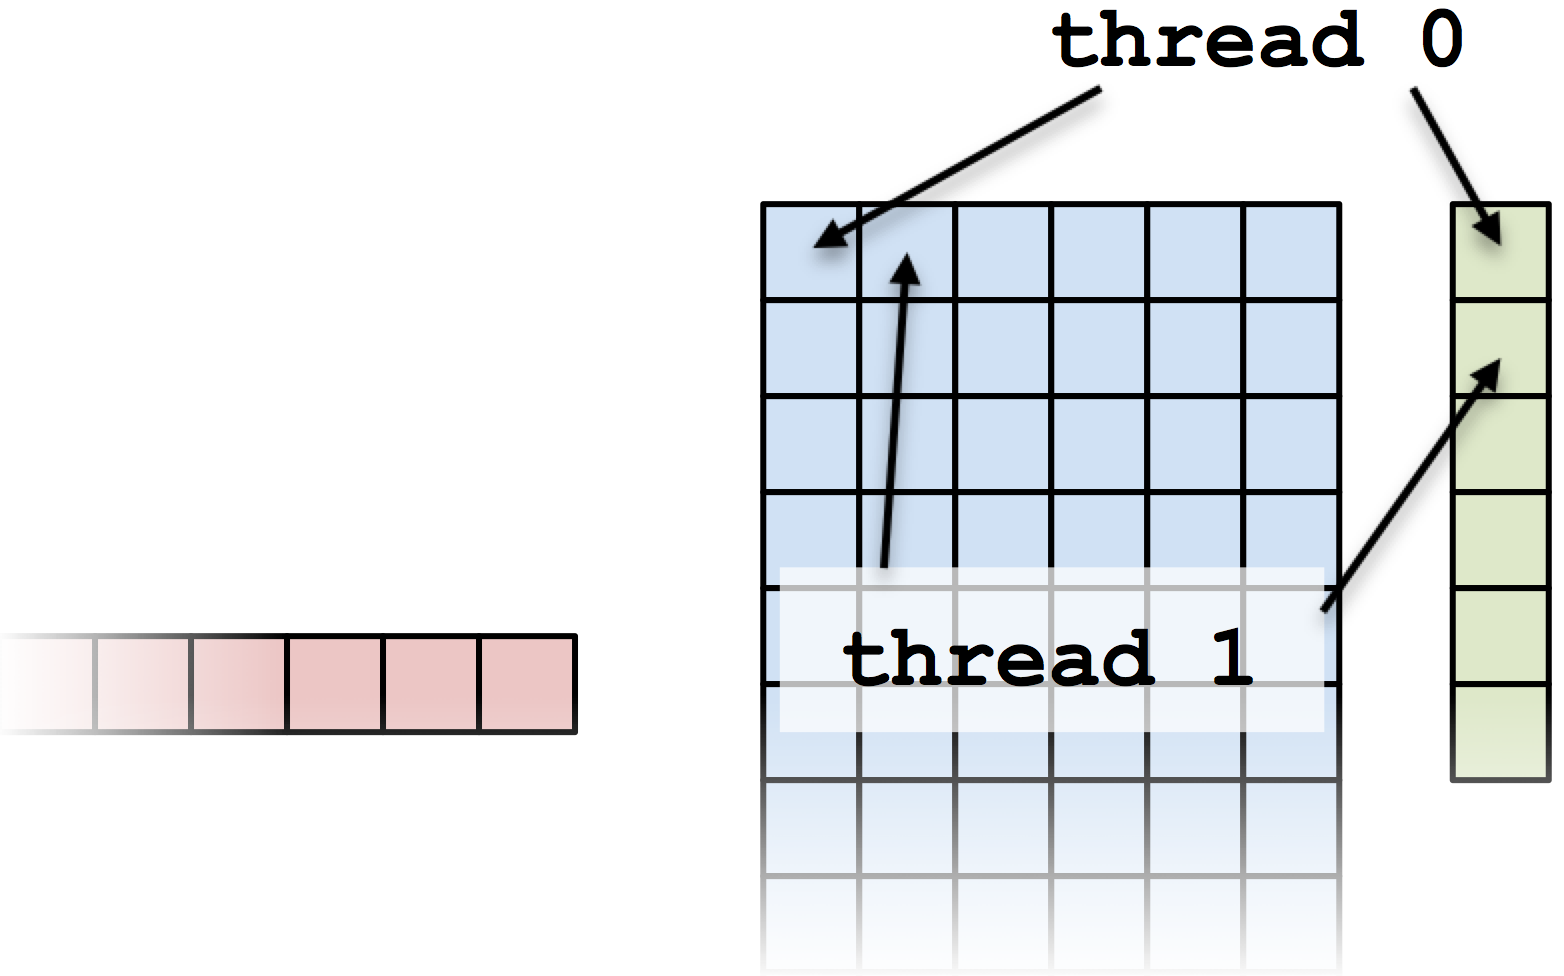
\includegraphics[width=0.60\textwidth]{figures/InnerProductExample_Atomics}
      \end{tikzpicture}
      };
  \end{tikzpicture}

  \vspace{10pt}
  \pause

  \begin{columns}[t,onlytextwidth]
    \column{.60\textwidth}
    {\color{red}\textbf{Problem:}} Poor performance
    \column{.40\textwidth}
  \end{columns}

  \vspace{50pt}

\end{frame}
\fi

%==========================================================================

\begin{frame}[fragile]{Example: inner product (2)}

  Using an atomic with every element is doing scalar integration with atomics.  (See module 3)

  \vspace{10pt}

  Instead, you could envision doing a large number of \texttt{parallel\_reduce} kernels.

  \begin{code}[keywords={}]
for each row
  Functor functor(row, ...);
  parallel_reduce(M, functor);
}
  \end{code}

  \vspace{10pt}
  \pause

  This is an example of \emph{hierarchical work}.

  \begin{block}{Important concept: Hierarchical parallelism}
    Algorithms that exhibit hierarchical structure can exploit hierarchical parallelism with \textbf{thread teams}.
  \end{block}

\end{frame}

%==========================================================================

\ifmedium
\begin{frame}[fragile]{Example: inner product (3)}

  \begin{block}{Important concept: Thread team}
  A collection of threads which are guaranteed to be executing \textbf{concurrently} and \textbf{can synchronize}.
  \end{block}

  \pause
  \vspace{-15pt}

 \begin{tikzpicture}[remember picture, overlay]
    \node [shift={(-6.0cm,0.75cm)}]  at (current page.south east)
      {%
      \begin{tikzpicture}[remember picture, overlay]
        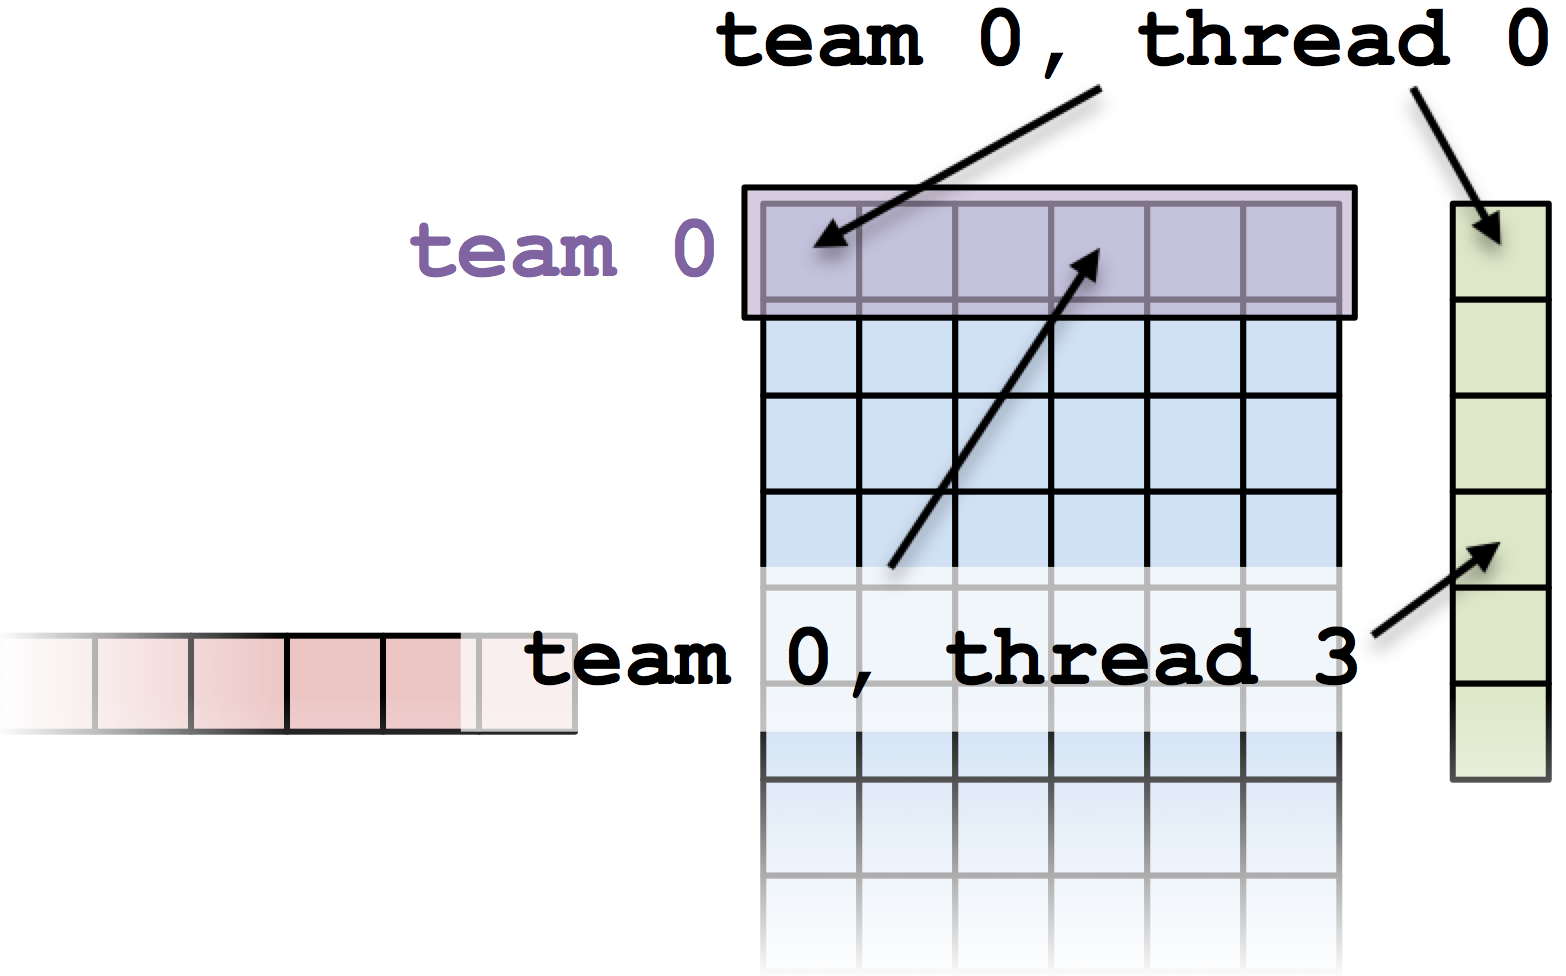
\includegraphics[width=0.53\textwidth]{figures/InnerProductExample_Teams}
      \end{tikzpicture}
      };
  \end{tikzpicture}

  High-level \textbf{strategy}:

  \vspace{-3pt}

  \begin{enumerate}
    \item{Do \textbf{one parallel launch} of \texttt{N} teams.}
    \item{Each team handles a row.}
    \item{The threads within \textbf{teams perform a reduction}.}
    \item{The thread teams \textbf{perform a reduction}.}
  \end{enumerate}

  %\vspace{-15pt}
  \vspace{85pt}

  %\begin{center}
    %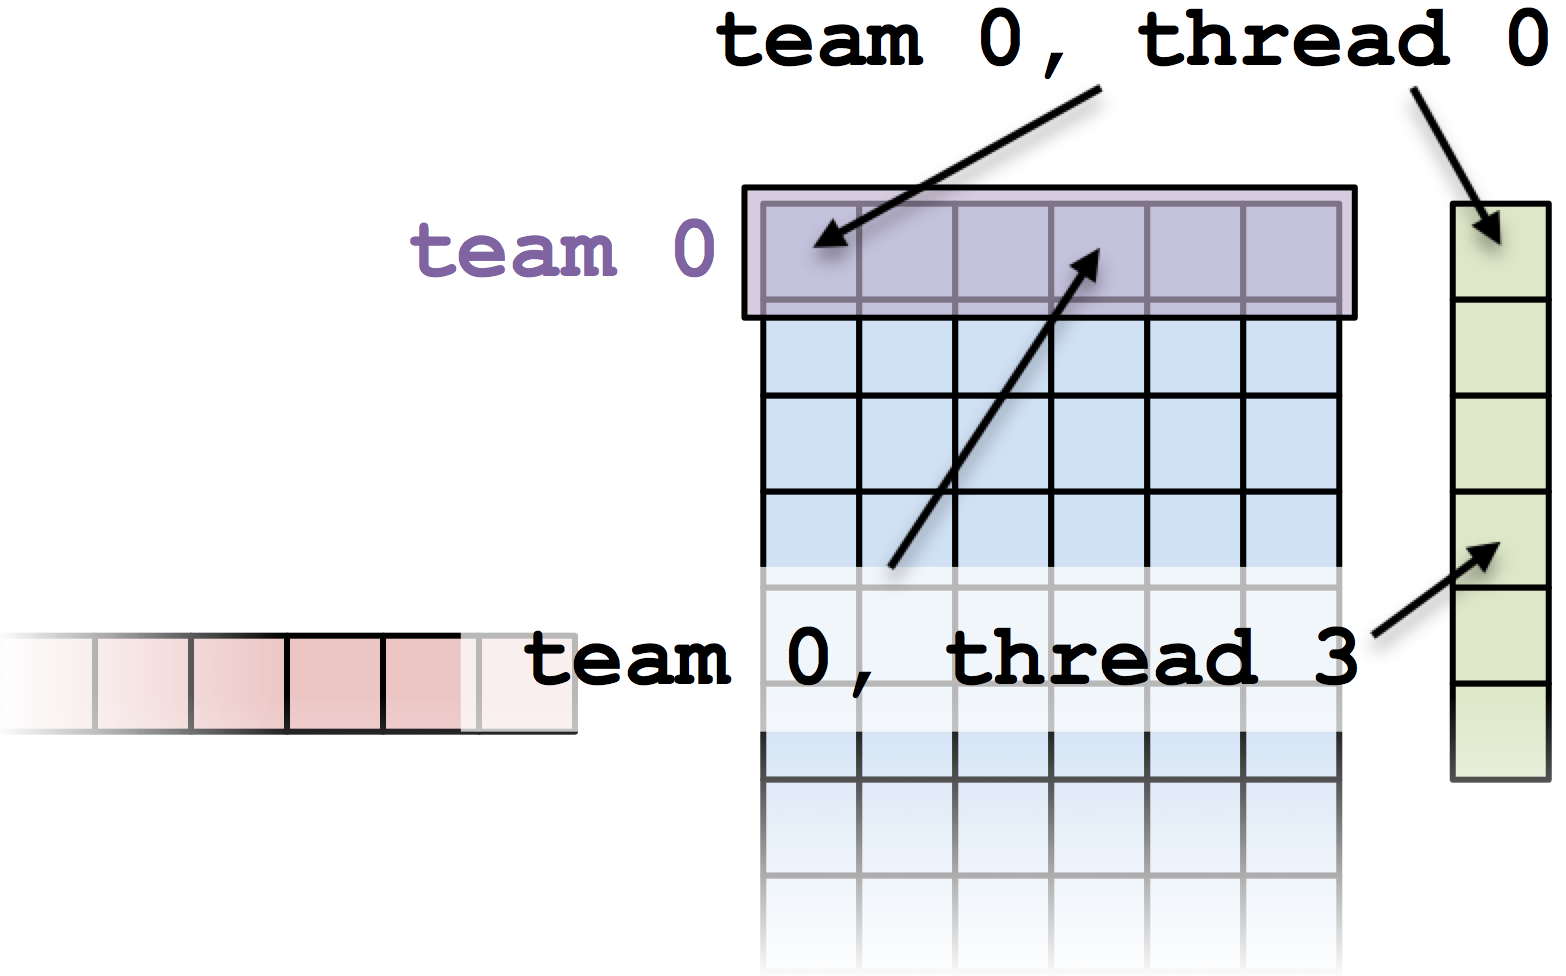
\includegraphics[width=0.40\textwidth]{figures/InnerProductExample_Teams}
  %\end{center}

  %\vspace{-5pt}

\end{frame}
\fi

%==========================================================================

\ifmedium
\begin{frame}[fragile]{Example: inner product (4)}

  \ul{\textbf{The \textit{final} hierarchical parallel kernel:}}

  \begin{code}
parallel_reduce("yAx",
  team_policy(N, Kokkos::AUTO),

  KOKKOS_LAMBDA (const member_type & @blueteamMember@blue, double & @orangeupdate@orange) {
    int @purplerow@purple = @blueteamMember@blue.league_rank();

    double thisRowsSum = 0;
    parallel_reduce(TeamThreadRange(@blueteamMember@blue, M),
      [=] (int @darkgreencol@darkgreen, double & @redinnerUpdate@red) {
        @redinnerUpdate@red += A(@purplerow@purple, @darkgreencol@darkgreen) * x(@darkgreencol@darkgreen);
      }, thisRowsSum);

    if (@blueteamMember@blue.team_rank() == 0) {
      update += y(@purplerow@purple) * thisRowsSum;
    }
  }, @orangeresult@orange);
  \end{code}

  %\vspace{5pt}

  %The \textbf{performance} and \textbf{flexibility} of teams is \emph{naturally} and \emph{concisely} expressed under the Kokkos model.

  %\vspace{1em}

  %Let's walk through how we got to this \textit{final} answer.

\end{frame}
\fi

%==========================================================================

\begin{frame}[fragile]{TeamPolicy (0)}

  \begin{block}{Important point}
    Using teams is changing the execution \emph{policy}.
  \end{block}

  \vspace{10pt}

  ``\textbf{Flat} parallelism'' uses \texttt{RangePolicy}:

  \vspace{3pt}

  \hspace{20pt}We specify a \emph{total amount of work}.

  \vspace{0pt}

  \begin{code}
// total work = N
@patternparallel_for@pattern("Label", 
  @policyRangePolicy<ExecutionSpace>(0,N)@policy, @bodyfunctor@body);
  \end{code}

  \pause
  \vspace{15pt}
  ``\textbf{Hierarchical} parallelism'' uses \texttt{TeamPolicy}:

  \vspace{3pt}

  \hspace{20pt}We specify a \emph{team size} and a \emph{number of teams}.

  \begin{code}[linebackgroundcolor={
      },
      keywords={}
    ]
// total work = numberOfTeams * teamSize
@patternparallel_for@pattern("Label", 
  @policyTeamPolicy<ExecutionSpace>(numberOfTeams, teamSize)@policy, @bodyfunctor@body);
  \end{code}

  \vspace{10pt}
\end{frame}

%==========================================================================

\begin{frame}[fragile]{TeamPolicy (1)}

  \begin{block}{Important point}
    When using teams, functor operators receive a \emph{team member}.
  \end{block}

  \begin{code}[linebackgroundcolor={
      },
      keywords={}
    ]
using member_type = typename TeamPolicy<ExecSpace>::member_type;

void operator()(const member_type & teamMember) {
  <@{\bf // How many teams are there?}@>
  const unsigned int league_size = teamMember.league_size();

  <@{\bf // Which team am I on?}@>
  const unsigned int league_rank = teamMember.league_rank();

  <@{\bf // How many threads are in the team?}@>
  const unsigned int team_size = teamMember.team_size();

  <@{\bf // Which thread am I on this team?}@>
  const unsigned int team_rank = teamMember.team_rank();

  <@{\bf // Make threads in a team wait on each other:}@>
  teamMember.team_barrier();
}
  \end{code}

\end{frame}


%==========================================================================

\iffull
\begin{frame}[fragile]{\texttt{TeamThreadRange} (0)}

 \begin{tikzpicture}[remember picture, overlay]
    \node [shift={(-6.0cm,-4.70cm)}]  at (current page.north east)
      {%
      \begin{tikzpicture}[remember picture, overlay]
        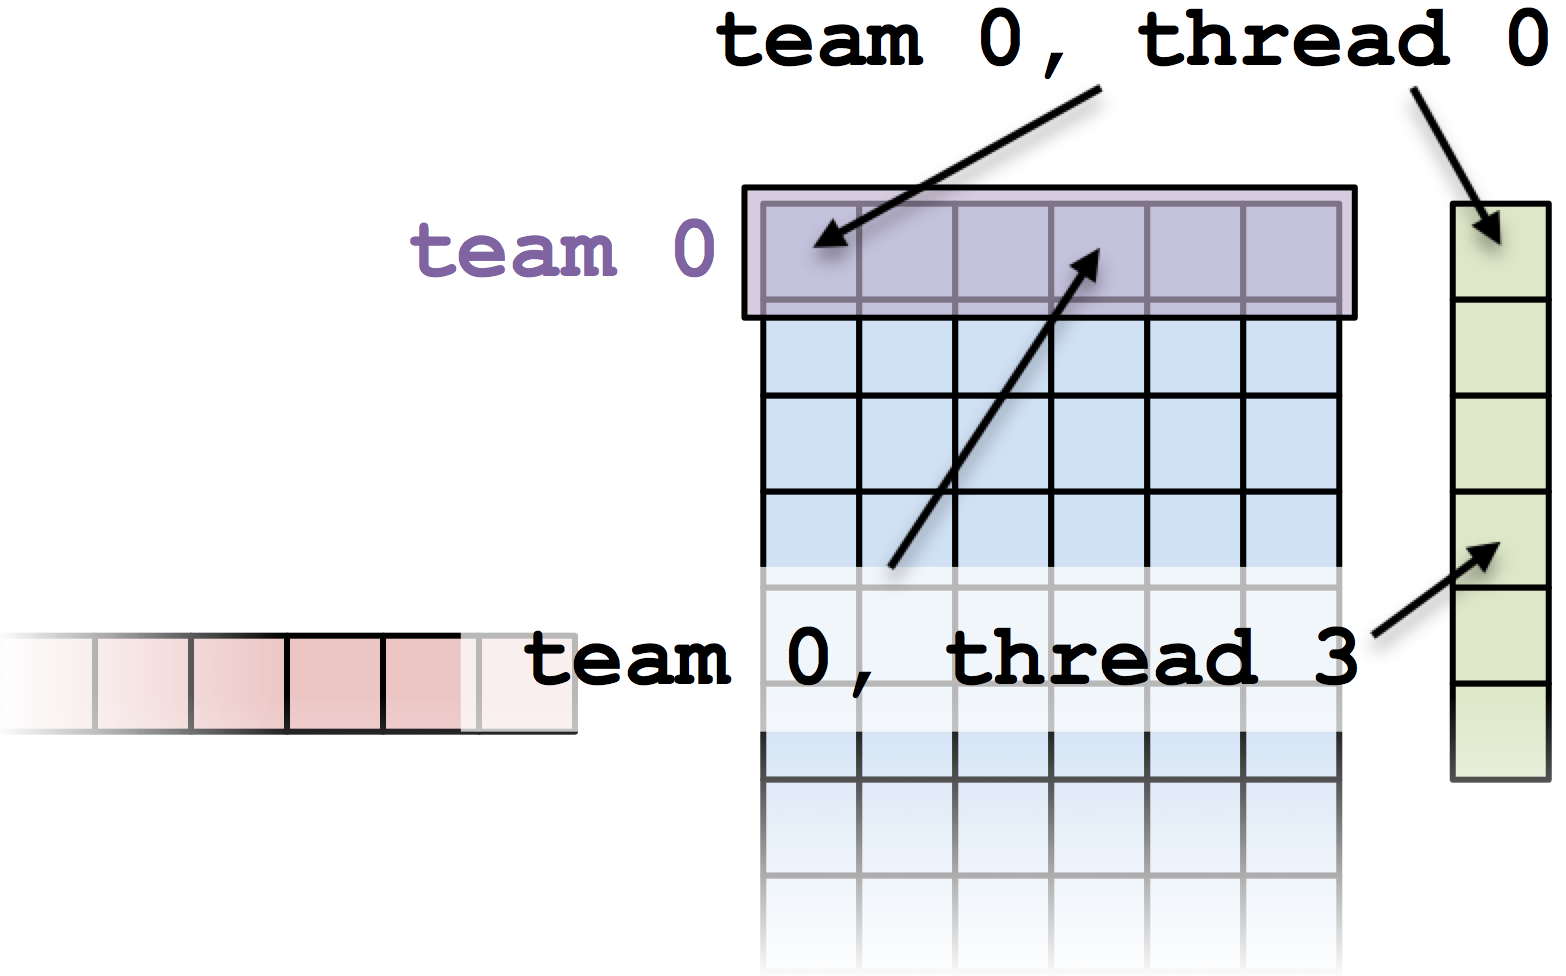
\includegraphics[width=0.53\textwidth]{figures/InnerProductExample_Teams}
      \end{tikzpicture}
      };
  \end{tikzpicture}

  \vspace{50pt}

  First attempt at exercise:

  \begin{code}
@grayoperator() (member_type & teamMember ) {
  const size_t row = teamMember.league_rank();
  const size_t col = teamMember.team_rank();@gray
  atomic_add(&@orangeresult@orange,@darkredy@darkred(row) * @blueA@blue(row,col) * @darkgreenx@darkgreen(entry));
@gray}@gray
  \end{code}

  \pause
  \vspace{-5pt}

  \begin{itemize}

  \item {When team size $\neq$ number of columns, how are units of work mapped to team's member threads?  Is the mapping architecture-dependent?}

  \end{itemize}

\end{frame}
\fi

%==========================================================================

\iffull
\begin{frame}[fragile]{\texttt{TeamThreadRange} (1)}


  Second attempt at exercise:

\vspace{10pt}
  Divide row length among team members.

  \begin{code}
@grayoperator() (member_type & teamMember ) {
  const size_t row = teamMember.league_rank();

  int begin = teamMember.team_rank();
  for(int col = begin; col < M; col += teamMember.team_size()) {
    atomic_add(&@orangeresult@orange, @darkredy@darkred(row) * @blueA@blue(row,col) * @darkgreenx@darkgreen(entry));
  }
@gray}@gray
  \end{code}

  \pause
  \vspace{-5pt}

  \begin{itemize}

  \item {Still bad because \texttt{atomic\_add} performs badly under high contention, how can team's member threads performantly cooperate for a nested reduction?}

  \item {On CPUs you get a bad data access pattern: this hardcodes coalesced access, but not caching.}

  \end{itemize}

\end{frame}
\fi

%==========================================================================

\begin{frame}[fragile]{\texttt{TeamThreadRange} (2)}

  We shouldn't be hard-coding the work mapping...

  \begin{code}[linebackgroundcolor={
        \btLstHL<1->{6}{bodyColor}
      },
      keywords={}
    ]
@grayoperator() (member_type & teamMember, double & update) {
  const int row = teamMember.league_rank();@gray
  double @purplethisRowsSum@purple;
  @pattern``do a reduction''@pattern(@policy``over M columns''@policy,
    [=] (const int col) {
      @purplethisRowsSum@purple += @blueA@blue(row,col) * @darkgreenx@darkgreen(col);
    });
  if (teamMember.team_rank() == 0) {
    update += @darkred@darkred(row) * @purplethisRowsSum@purple;
  }
@gray}@gray
  \end{code}

  \pause
  \vspace{5pt}

  If this were a parallel execution, \\
    \hspace{20pt}we'd use \texttt{Kokkos::parallel\_reduce}.

  \pause
  \vspace{5pt}

  \textbf{Key idea}: this \emph{is} a parallel execution.

  \pause
  \vspace{5pt}

  \hspace{20pt}{\Large $\Rightarrow$ \textbf{Nested parallel patterns}}

\end{frame}

%==========================================================================

\begin{frame}[fragile]{\texttt{TeamThreadRange} (3)}

  \ul{\texttt{TeamThreadRange}:}

  \begin{code}[linebackgroundcolor={
        \btLstHL<1->{6}{bodyColor}
      },
      keywords={}
    ]
@grayoperator() (const member_type & teamMember, double & update ) {
  const int row = teamMember.league_rank();@gray
  double @purplethisRowsSum@purple;
  @patternparallel_reduce@pattern(@policyTeamThreadRange(teamMember, M)@policy,
    [=] (const int col, double & thisRowsPartialSum ) {
      thisRowsPartialSum += @blueA@blue(row, col) * @darkgreenx@darkgreen(col);
    }, @purplethisRowsSum@purple );
  if (teamMember.team_rank() == 0) {
    update += @darkredy@darkred(row) * @purplethisRowsSum@purple;
  }
@gray}@gray
  \end{code}

  \pause

  \begin{itemize}
    \item{The \textbf{mapping} of work indices to threads is \textbf{architecture-dependent}.}
    \item{The \textbf{amount of work} given to the \texttt{TeamThreadRange} \textbf{need not be a multiple} of the \texttt{team\_size}.}
    \item{Intrateam \textbf{reduction handled} by Kokkos.}
  \end{itemize}

\end{frame}

%==========================================================================

\begin{frame}[fragile]{Nested parallelism}

  \ul{\textbf{Anatomy} of nested parallelism:}

  \vspace{-3pt}

  \begin{code}[linebackgroundcolor={
        %\btLstHL<1->{4-7}{bodyColor}
      },
      keywords={}
    ]
@patternparallel_outer@pattern("Label",
  @policyTeamPolicy<ExecutionSpace>(numberOfTeams, teamSize)@policy,
  KOKKOS_LAMBDA (const member_type & teamMember@italic[, ...]@italic) {
    /* beginning of outer body */
    @patternparallel_inner@pattern(
      @policyTeamThreadRange(teamMember, thisTeamsRangeSize)@policy,
      [=] (const unsigned int indexWithinBatch@italic[, ...]@italic) {
        /* inner body */
      }@italic[, ...]@italic);
    /* end of outer body */
  }@italic[, ...]@italic);
  \end{code}

  \vspace{-5pt}

  \begin{itemize}
    \item{\texttt{parallel\_outer} and \texttt{parallel\_inner} may be any combination of \texttt{for} and/or \texttt{reduce}.}
    \item{The inner lambda may capture by reference, but capture-by-value is recommended.}
    \item{The policy of the inner lambda is always a \texttt{TeamThreadRange}.}
    \item{\texttt{TeamThreadRange} cannot be nested.}
  \end{itemize}

\end{frame}

%==========================================================================

\begin{frame}[fragile]{What should the team size be?}

  In practice, you can \textbf{let Kokkos decide}:

    \begin{code}[linebackgroundcolor={
      },
      keywords={}
    ]
parallel_something(
  TeamPolicy<ExecutionSpace>(numberOfTeams, Kokkos::AUTO),
  /* functor */);
    \end{code}

  \pause
  \vspace{0pt}

  \ul{\textbf{GPUs}}

  \begin{itemize}
    \item{Special hardware available for coordination within a team.}
    \item{Within a team 32 (NVIDIA) or 64 (AMD) threads execute ``lock step.''}
    \item{Maximum team size: \textbf{1024}; Recommended team size: \textbf{128/256}}
  \end{itemize}

  \pause
  \vspace{0pt}

  \ul{\textbf{Intel Xeon Phi}:}

  \begin{itemize}
    \item{Recommended team size: \# hyperthreads per core}
    \item{Hyperthreads share entire cache hierarchy} \\
      \hspace{2em}{a well-coordinated team avoids cache-thrashing}
  \end{itemize}

\end{frame}

%==========================================================================

\begin{frame}[fragile]{Exercise: TeamPolicy}

  \textbf{Details}:
  \begin{small}
  \begin{itemize}
\item Location: \ExerciseDirectory{team\_policy}
\item Replace \texttt{RangePolicy<Space>} with \texttt{TeamPolicy<Space>}
\item Use \texttt{AUTO} for \texttt{team\_size}
\item Make the inner loop a \texttt{parallel\_reduce} with \texttt{TeamThreadRange} policy
\item Experiment with the combinations of \texttt{Layout}, \texttt{Space}, \texttt{N} to view performance
\item Hint: what should the layout of \texttt{A} be?
\end{itemize}
  \end{small}

\ul{\textbf{Things to try:}}
  \begin{small}
  \begin{itemize}
  \item Vary problem size and number of rows (-S ...; -N ...)
  \item Compare behavior with Exercise 4 for very non-square matrices
  \item Compare behavior of CPU vs GPU
  \end{itemize}
  \end{small}

\end{frame}

%==========================================================================

\begin{frame}[fragile]{Reminder, Exercise \#4 with Flat Parallelism}

  \vspace{-5pt}
  \hspace{-15pt}
    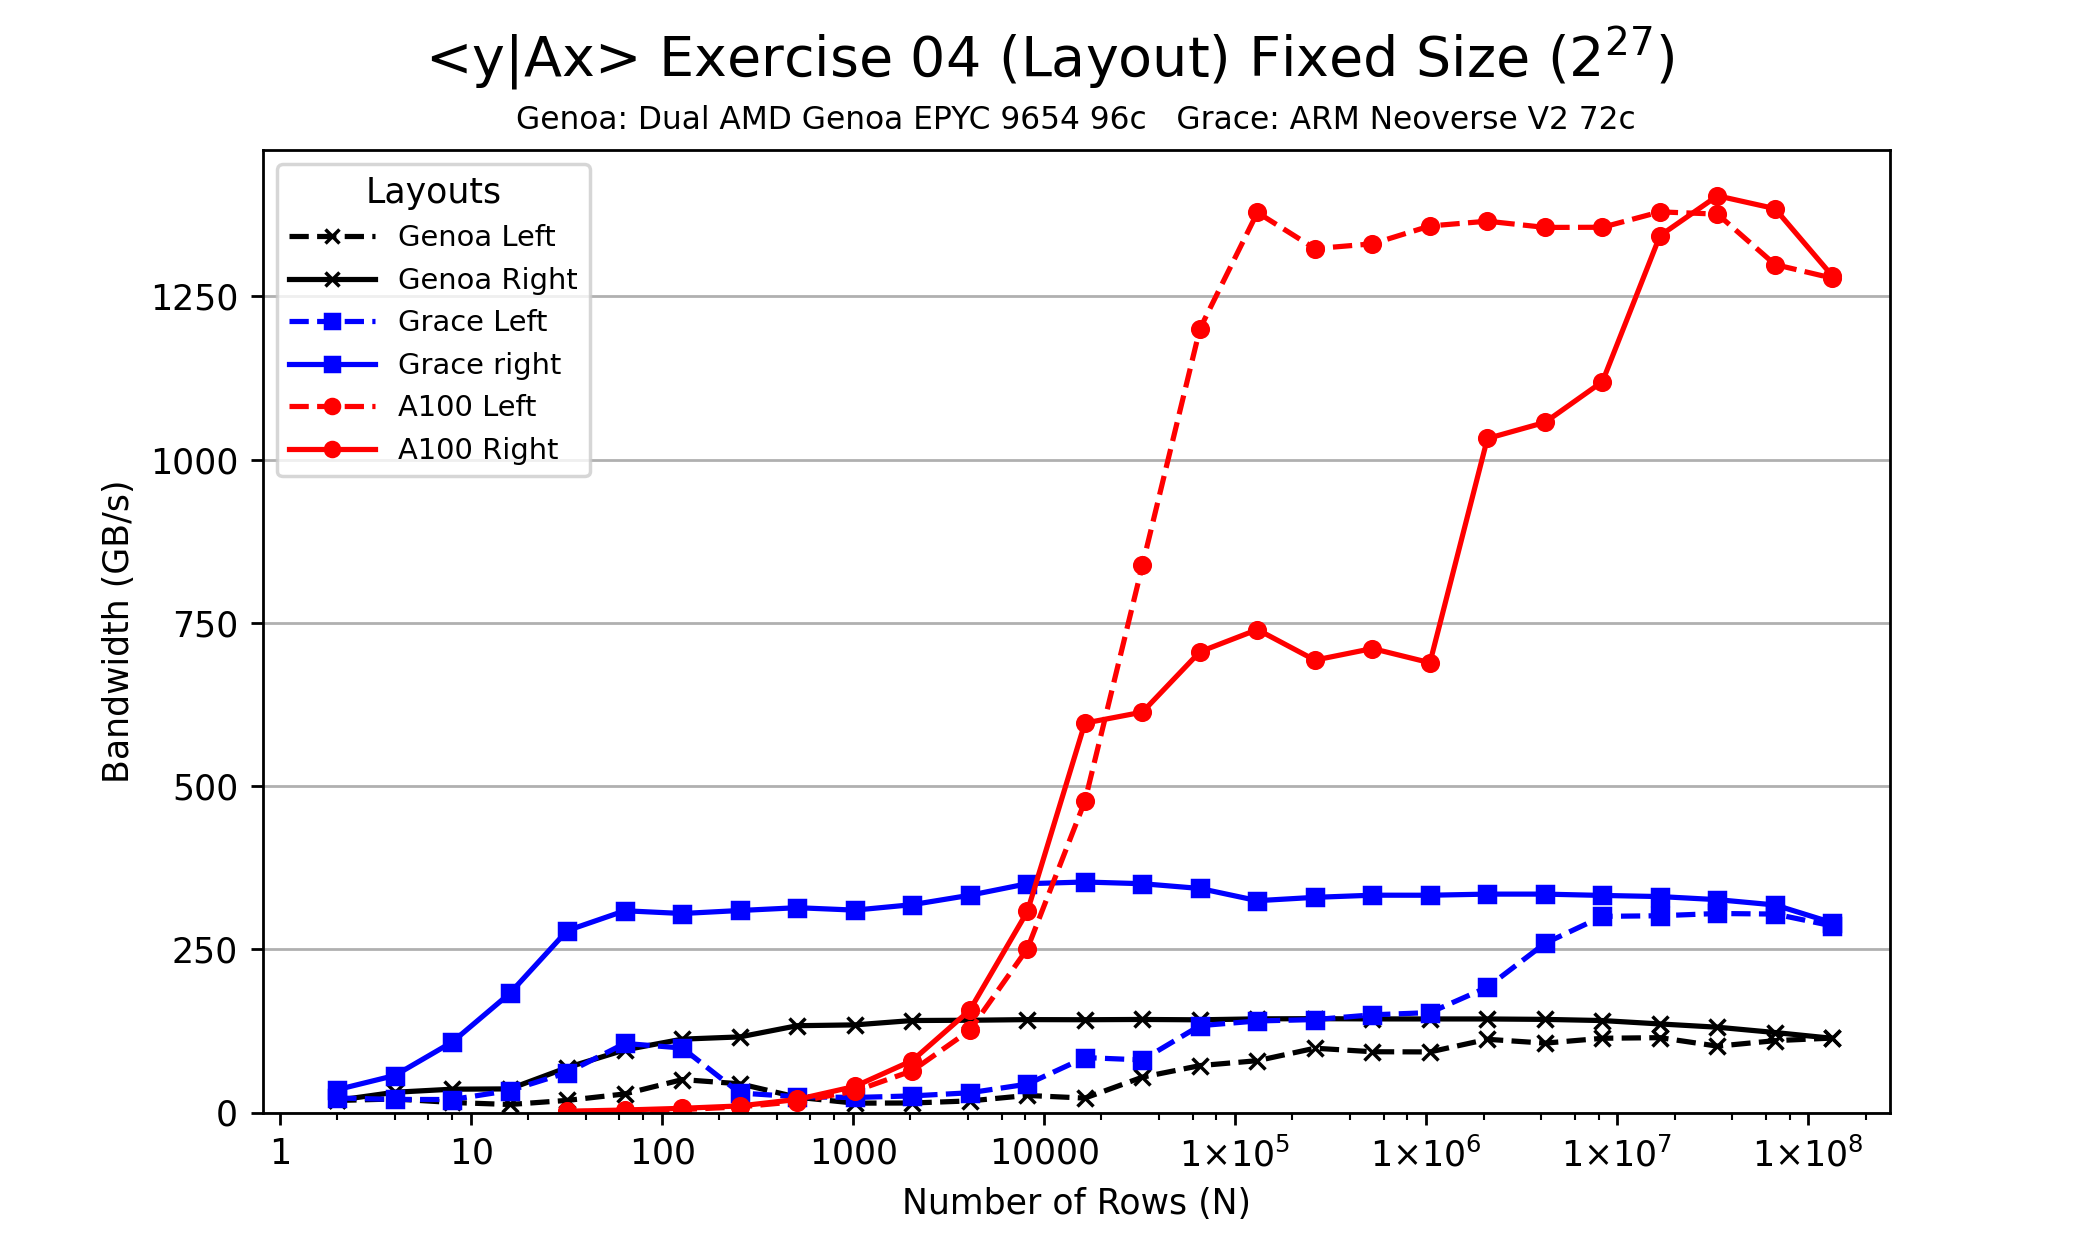
\includegraphics[trim=20pt 0 50pt 5pt, clip, width=1.0\textwidth]{figures/Exercise04-Performance.png}
  \vspace{-15pt}

  \begin{textblock*}{0.5\textwidth}(0.69\textwidth,0.30\textheight)
    \textbf{coalesced}
  \end{textblock*}

  \begin{textblock*}{0.5\textwidth}(0.35\textwidth,0.65\textheight)
    \textbf{cached}
  \end{textblock*}

  \begin{textblock*}{0.5\textwidth}(0.65\textwidth,0.56\textheight)
    \textbf{uncoalesced}
  \end{textblock*}

  \begin{textblock*}{0.5\textwidth}(0.71\textwidth,0.78\textheight)
    \textbf{uncached}
  \end{textblock*}

\end{frame}

%==========================================================================

\begin{frame}[fragile]{Exercise: TeamPolicy}

  \vspace{-10pt}

  \begin{center}
    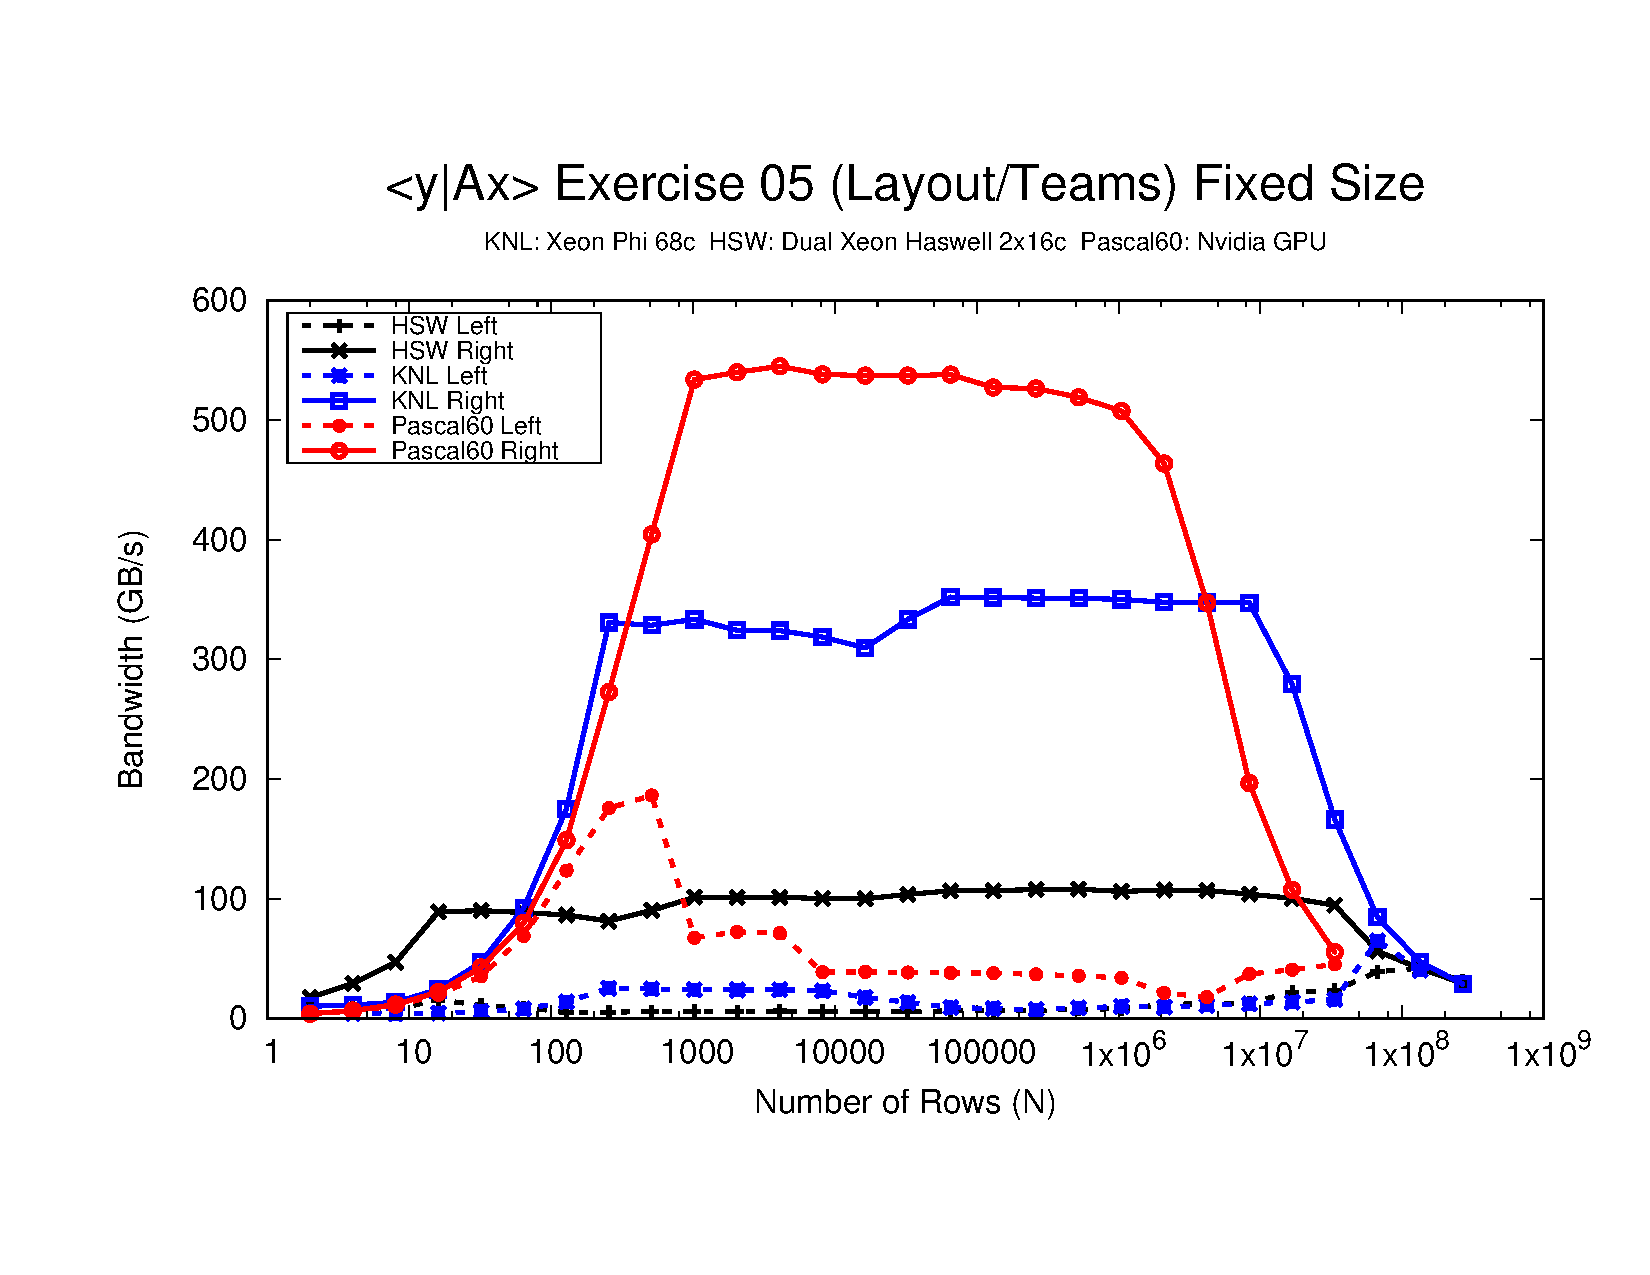
\includegraphics[viewport=1.25in 3.0in 10in 6in, width=0.95\textwidth]{figures/Exercise05-Performance.pdf}
  \end{center}

  \vspace{-15pt}

  \begin{textblock*}{0.5\textwidth}(0.55\textwidth,0.32\textheight)
    \textbf{coalesced}
  \end{textblock*}

  \begin{textblock*}{0.5\textwidth}(0.60\textwidth,0.44\textheight)
    \textbf{cached}
  \end{textblock*}

  \begin{textblock*}{0.5\textwidth}(0.70\textwidth,0.68\textheight)
    \textbf{cached}
  \end{textblock*}

\end{frame}

%==========================================================================

\begin{comment}
\begin{frame}[fragile]{Example: sparse matrix-vector product (0)}

  Sparse matrix \textbf{representation}:

  \vspace{-7pt}

  \begin{table}
    \small
    \begin{tabular}{| l | c | c | c | c | c |}
      \hline
      \texttt{colIndices} & 17 & 45 & 73 & 7 & ... \\
      \hline
      \texttt{colValues} & 3.1 & 4.1 & 5.9 & 2.6 & ...\\
      \hline
      \texttt{irow} & 0 & 3 & 9 & ... & \\
      \hline
    \end{tabular}
  \end{table}

  \vspace{10pt}

  \textbf{Serial} algorithm:

  \vspace{-2pt}

  \begin{code}[linebackgroundcolor={
      },
      keywords={}
    ]
for (row = 0; row < matrixSize; ++row) {
  double total = 0;
  for (int i = irow[row]; i < irow[row+1]; ++i) {
    total += colValues[i] * vec[colIndices[i]];
  }
  product[row] = total;
}
  \end{code}

  \pause
  \vspace{10pt}

  How many ways can this be parallelized?

\end{frame}

%==========================================================================

\begin{frame}[fragile]{Example: sparse matrix-vector product (1)}

  \ul{\textbf{Flat} over \textbf{rows}:}

  \begin{code}[linebackgroundcolor={
      },
      frame=single,
      keywords={}
    ]
operator()(int row) const {
  double total = 0;
  for (int i = _irow(row); i < _irow(row+1); ++i) {
    total += _colValues(i) * _vec(_colIndices(i));
  }
  _product[row] = total;
}
  \end{code}

  \vspace{5pt}

  \begin{itemize}
    \item{One thread \textbf{per row}}
    \item{\texttt{\_colValues} and \texttt{\_colIndices}: {\color{darkgreen}cached}/{\color{darkred}uncoalesced}}
    \item{\texttt{\_vec}: {\color{darkred}uncached}/{\color{darkred}uncoalesced}}
    \item{\texttt{\_product}: {\color{darkgreen}cached}/{\color{darkgreen}coalesced}}
  \end{itemize}

\end{frame}

%==========================================================================

\begin{frame}[fragile]{Example: sparse matrix-vector product (2)}

  \ul{\textbf{Flat} over \textbf{non-zeros} with atomics:}

  \begin{code}[linebackgroundcolor={
      },
      frame=single,
      keywords={}
    ]
operator()(int i) const {
  atomic_add(&_product(_rowIndices(i)),
             colValues(i) * _vec(_colIndices(i)));
}
  \end{code}

  \begin{itemize}
    \item{One thread \textbf{per nonzero entry}}
    \item{\texttt{\_colValues}, \texttt{\_colIndices}, \texttt{\_rowIndices}: {\color{darkgreen}cached}/{\color{darkgreen}coalesced}}
    \item{\texttt{\_vec}: {\color{darkred}uncached}/{\color{darkred}uncoalesced}}
    \item{\texttt{\_product}: {\color{darkgreen}good}/{\color{darkred}bad}}
  \end{itemize}

\end{frame}

%==========================================================================

\begin{frame}[fragile]{Example: sparse matrix-vector product (3)}

  \ul{Hierarchical \textbf{thread teams}:}

  \begin{code}[linebackgroundcolor={
      },
      frame=single,
      keywords={}
    ]
operator()(member_type teamMember) const {
  int row = teamMember.league_rank();
  double total;
  Kokkos::parallel_reduce
    (Kokkos::TeamThreadRange(teamMember, numNonzeros),
     [=] (const unsigned int j, double & valueToUpdate) {
      const unsigned int i = irow(row) + j;
      valueToUpdate += _colValues(i) * _vec(_colIndices(i));
    }, total);
  if (teamMember.team_rank() == 0) {
    _product(row) = total;
  }
}
  \end{code}

  \vspace{-5pt}

  \begin{itemize}
    \item{One thread \textbf{per nonzero entry}}
    \item{\texttt{\_colValues}, \texttt{\_colIndices}: {\color{darkgreen}cached}/{\color{darkgreen}coalesced}}
    \item{\texttt{\_vec}: {\color{darkred}uncached}/{\color{darkred}uncoalesced}}
    \item{\texttt{\_product}: {\color{darkgreen}cached}/{\color{darkgreen}single write}}
  \end{itemize}

\end{frame}

%==========================================================================

\begin{frame}[fragile]{Example: sparse matrix-vector product (4)}

  \ul{\textbf{Performance:}}

  \begin{center}
    \includegraphics[width=1.00\textwidth]{figures/SparseMatrixVectorProduct_summaryNoTexture.pdf}
  \end{center}

\end{frame}

%==========================================================================

\begin{frame}[fragile]{Example: sparse matrix-vector product (5)}

  \ul{\textbf{Performance} (including texture versions):}

  \begin{center}
    \includegraphics[width=1.00\textwidth]{figures/SparseMatrixVectorProduct_summary.pdf}
  \end{center}

\end{frame}
\end{comment}

%==========================================================================

\begin{frame}[fragile]{Three-level parallelism (0)}

  \ul{\textbf{Exposing Vector Level Parallelism}}

  \begin{itemize}
    \item{Optional \textbf{third level} in the hierarchy: \texttt{ThreadVectorRange}}
      \begin{itemize}
        \item{Can be used for \texttt{parallel\_for}, \texttt{parallel\_reduce}, or \texttt{parallel\_scan}.}
      \end{itemize}
    \item{Maps to vectorizable loop on CPUs or (sub-)warp level parallelism on GPUs.}
    \item{Enabled with a \textbf{runtime} vector length argument to \texttt{TeamPolicy}}
    \item{There is \textbf{no} explicit access to a vector lane ID.}
    \item{Depending on the backend the full global parallel region has active vector lanes.}
    \item{\texttt{TeamVectorRange} uses both \textbf{thread} and \textbf{vector} parallelism.}
  \end{itemize}


\end{frame}

%==========================================================================

\begin{frame}[fragile]{Three-level parallelism (1)}

  \ul{\textbf{Anatomy} of nested parallelism:}

  \vspace{-3pt}

  \begin{code}[linebackgroundcolor={
        %\btLstHL<1->{4-7}{bodyColor}
      },
      keywords={}
    ]
@patternparallel_outer@pattern("Label",
  @policyTeamPolicy<>(numberOfTeams, teamSize, vectorLength)@policy,
  KOKKOS_LAMBDA (const member_type & teamMember@italic[, ...]@italic) {
    /* beginning of outer body */
    @patternparallel_middle@pattern(
      @policyTeamThreadRange(teamMember, thisTeamsRangeSize)@policy,
      [=] (const int indexWithinBatch@italic[, ...]@italic) {
        /* begin middle body */
        @patternparallel_inner@pattern(
           @policyThreadVectorRange(teamMember, thisVectorRangeSize)@policy,
           [=] (const int indexVectorRange@italic[, ...]@italic) {
             /* inner body */
           }@italic[, ....);
        /* end middle body */
      }@italic[, ...]@italic);
    @patternparallel_middle@pattern(
    @policyTeamVectorRange(teamMember, someSize)@policy,
      [=] (const int indexTeamVector[, ...]) {
	/* nested body */
      }[, ...]);
    /* end of outer body */
  }@italic[, ...]@italic);
  \end{code}

\end{frame}

%==========================================================================

\ifmedium
\begin{frame}[fragile]{Sum sanity checks (0)}

  \textbf{Question:} What will the value of \texttt{totalSum} be?

  \begin{code}[linebackgroundcolor={}]
int @darkgreentotalSum@darkgreen = 0;
parallel_reduce("Sum", RangePolicy<>(0, numberOfThreads),
  KOKKOS_LAMBDA (size_t& index, int& @darkredpartialSum@darkred) {
    int @bluethisThreadsSum@blue = 0;
    for (int i = 0; i < 10; ++i) {
      ++@bluethisThreadsSum@blue;
    }
    @darkredpartialSum@darkred += @bluethisThreadsSum@blue;
}, @darkgreentotalSum@darkgreen);
  \end{code}

  \pause

  \vspace{15pt}

  \texttt{totalSum = numberOfThreads * 10}

\end{frame}
\fi

%==========================================================================

\ifmedium
\begin{frame}[fragile]{Sum sanity checks (1)}

  \textbf{Question:} What will the value of \texttt{totalSum} be?

  \begin{code}[linebackgroundcolor={}]
@grayint totalSum = 0;
parallel_reduce("Sum", @grayTeamPolicy<>(numberOfTeams, team_size),
  @grayKOKKOS_LAMBDA (@graymember_type& teamMember,@gray int& partialSum) {
    int thisThreadsSum = 0;
    for (int i = 0; i < 10; ++i) {
      ++thisThreadsSum;
    }
    partialSum += thisThreadsSum;
}, totalSum);@gray
  \end{code}

  \pause

  \vspace{15pt}

  \texttt{totalSum = numberOfTeams * team\_size * 10}

\end{frame}
\fi

%==========================================================================

\ifmedium
\begin{frame}[fragile]{Sum sanity checks (2)}

  \textbf{Question:} What will the value of \texttt{totalSum} be?

  \begin{code}[linebackgroundcolor={}]
@grayint totalSum = 0;
parallel_reduce("Sum", TeamPolicy<>(numberOfTeams, team_size),
  KOKKOS_LAMBDA (member_type& teamMember, int& partialSum) {@gray
    int @orangethisTeamsSum@orange = 0;
    parallel_reduce(TeamThreadRange(teamMember, team_size),
      [=] (const int index, int& @purplethisTeamsPartialSum@purple) {
      @grayint thisThreadsSum = 0;
      for (int i = 0; i < 10; ++i) {
        ++thisThreadsSum;
      }@gray
      @purplethisTeamsPartialSum@purple += thisThreadsSum;
    }, @orangethisTeamsSum@orange);
    partialSum += @orangethisTeamsSum@orange;
@gray}, totalSum);@gray
  \end{code}

  \pause

  \vspace{15pt}

  \texttt{totalSum = numberOfTeams * team\_size * team\_size * 10}

\end{frame}
\fi

%==========================================================================

\begin{frame}[fragile]{Restricting Execution: single pattern}
The \texttt{single} pattern can be used to restrict execution
 \begin{itemize}
    \item{Like parallel patterns it takes a policy, a lambda, and optionally a broadcast argument.}
    \item{Two policies: \texttt{PerTeam} and \texttt{PerThread}.}
    \item{Equivalent to OpenMP {\bf single} directive with {\bf nowait}}
 \end{itemize}
\begin{code}[linebackgroundcolor={}]
// Restrict to once per thread
single(PerThread(teamMember), [&] () {
  // code
});

// Restrict to once per team with broadcast
int broadcastedValue = 0;
single(PerTeam(teamMember), [&] (int& broadcastedValue_local) {
	broadcastedValue_local = special value assigned by one;
}, broadcastedValue);
// Now everyone has the special value
\end{code}
\end{frame}

%==========================================================================

\begin{frame}[fragile]{Exercise: TeamVectorLoop}
The previous example was extended with an outer loop over ``Elements'' to expose
a third natural layer of parallelism.

\vspace{10pt}

  \textbf{Details}:
  \begin{small}
  \begin{itemize}
\item Location: \ExerciseDirectory{team\_vector\_loop}
\item Use the \texttt{single} policy instead of checking team rank
\item Parallelize all three loop levels.
\end{itemize}
  \end{small}

\ul{\textbf{Things to try:}}
  \begin{small}
  \begin{itemize}
  \item Vary problem size and number of rows (-S ...; -N ...)
  \item Compare behavior with TeamPolicy Exercise for very non-square matrices
  \item Compare behavior of CPU vs GPU
  \end{itemize}
  \end{small}
\end{frame}

%==========================================================================

\begin{frame}[fragile]{Exercise: TeamVectorLoop}

  %\vspace{-10pt}

    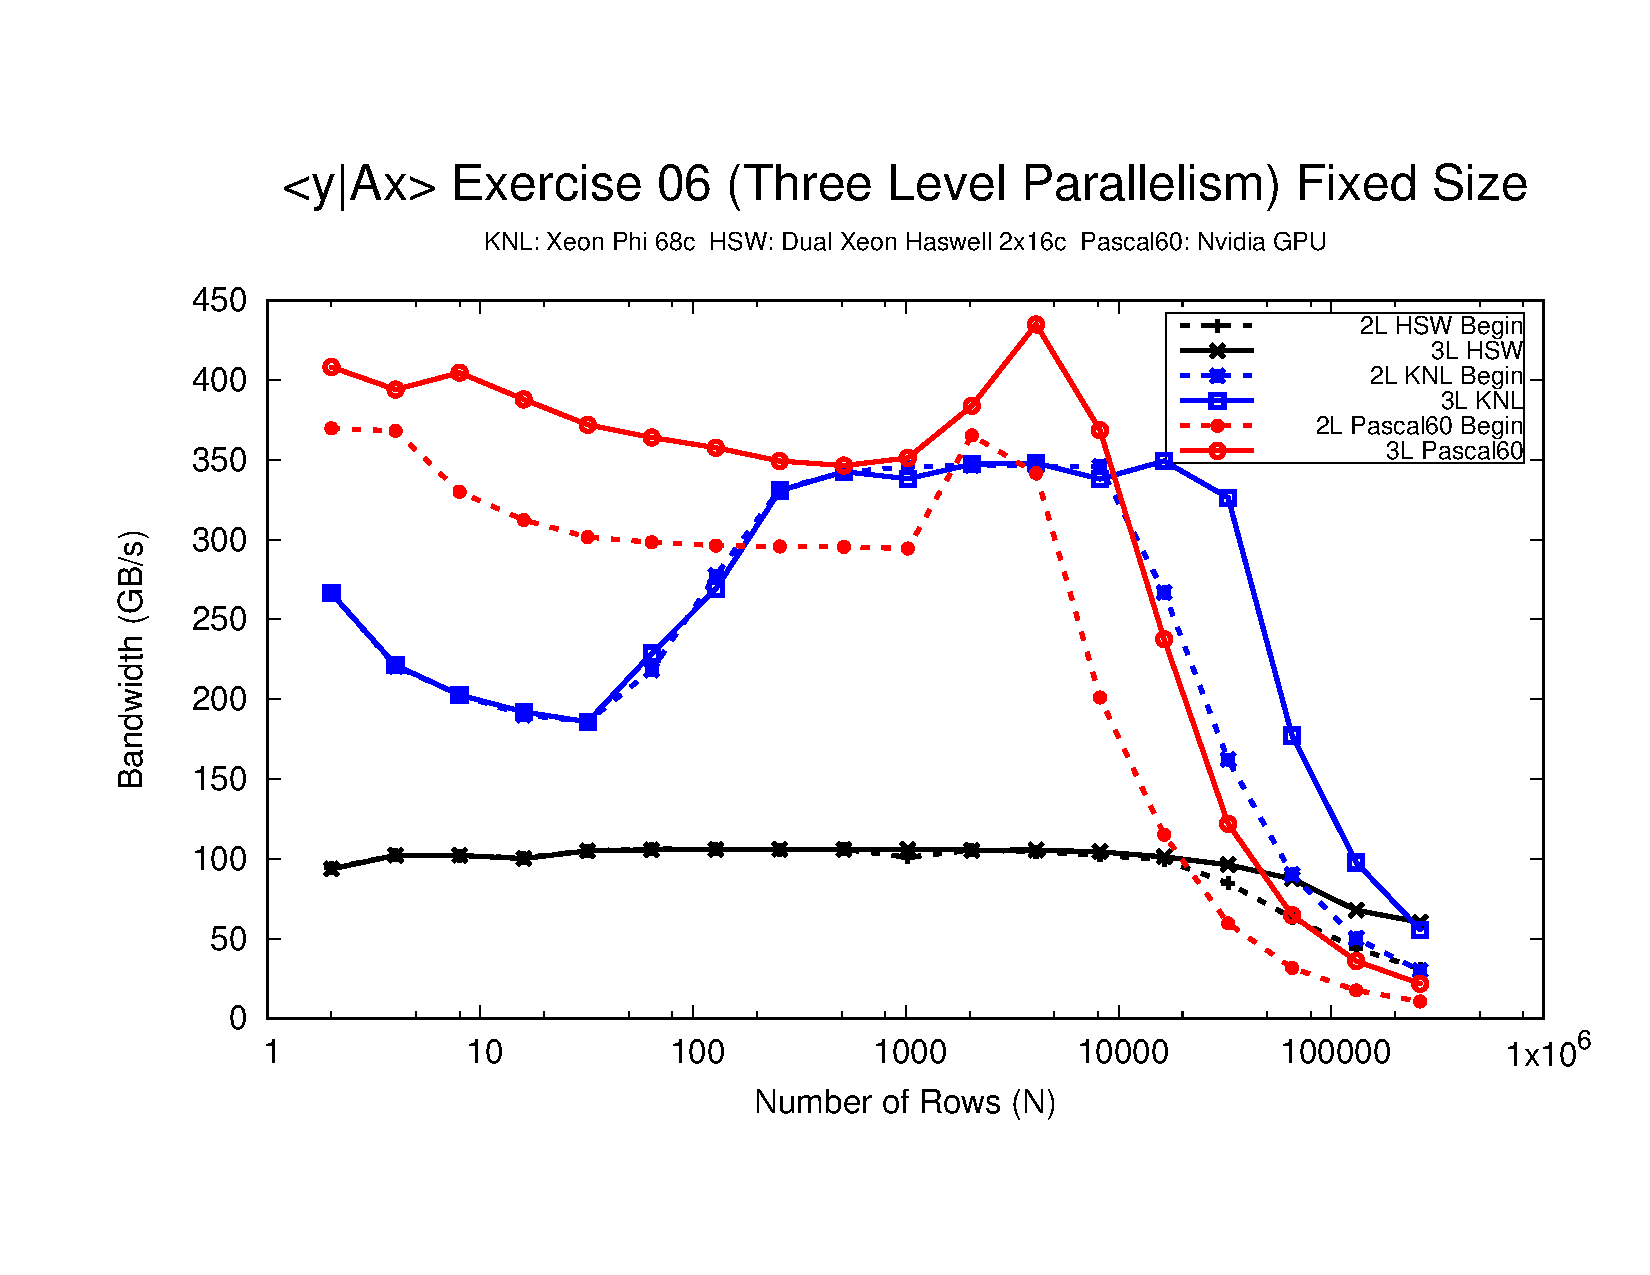
\includegraphics[viewport=1.25in 3.0in 10in 6in, width=0.95\textwidth]{figures/Exercise06-Performance.pdf}

  \vspace{-15pt}

\end{frame}

%==========================================================================

\begin{frame}{Section Summary}

  \begin{itemize}
    \item{\textbf{Hierarchical work} can be parallelized via hierarchical parallelism.}
    \item{Hierarchical parallelism is leveraged using \textbf{thread teams} launched with a \texttt{TeamPolicy}.}
    \item{Team ``worksets'' are processed by a team in nested \texttt{parallel\_for} (or \texttt{reduce} or \texttt{scan}) calls with a \texttt{TeamThreadRange}, \texttt{ThreadVectorRange}, and \texttt{TeamVectorRange} policy.}
    \item{Execution can be restricted to a subset of the team with the \texttt{single} pattern using either a \texttt{PerTeam} or \texttt{PerThread} policy.}
  \end{itemize}

\end{frame}
